% Describe the study area geography and climate

\begin{figure}[ht]
    \centering
    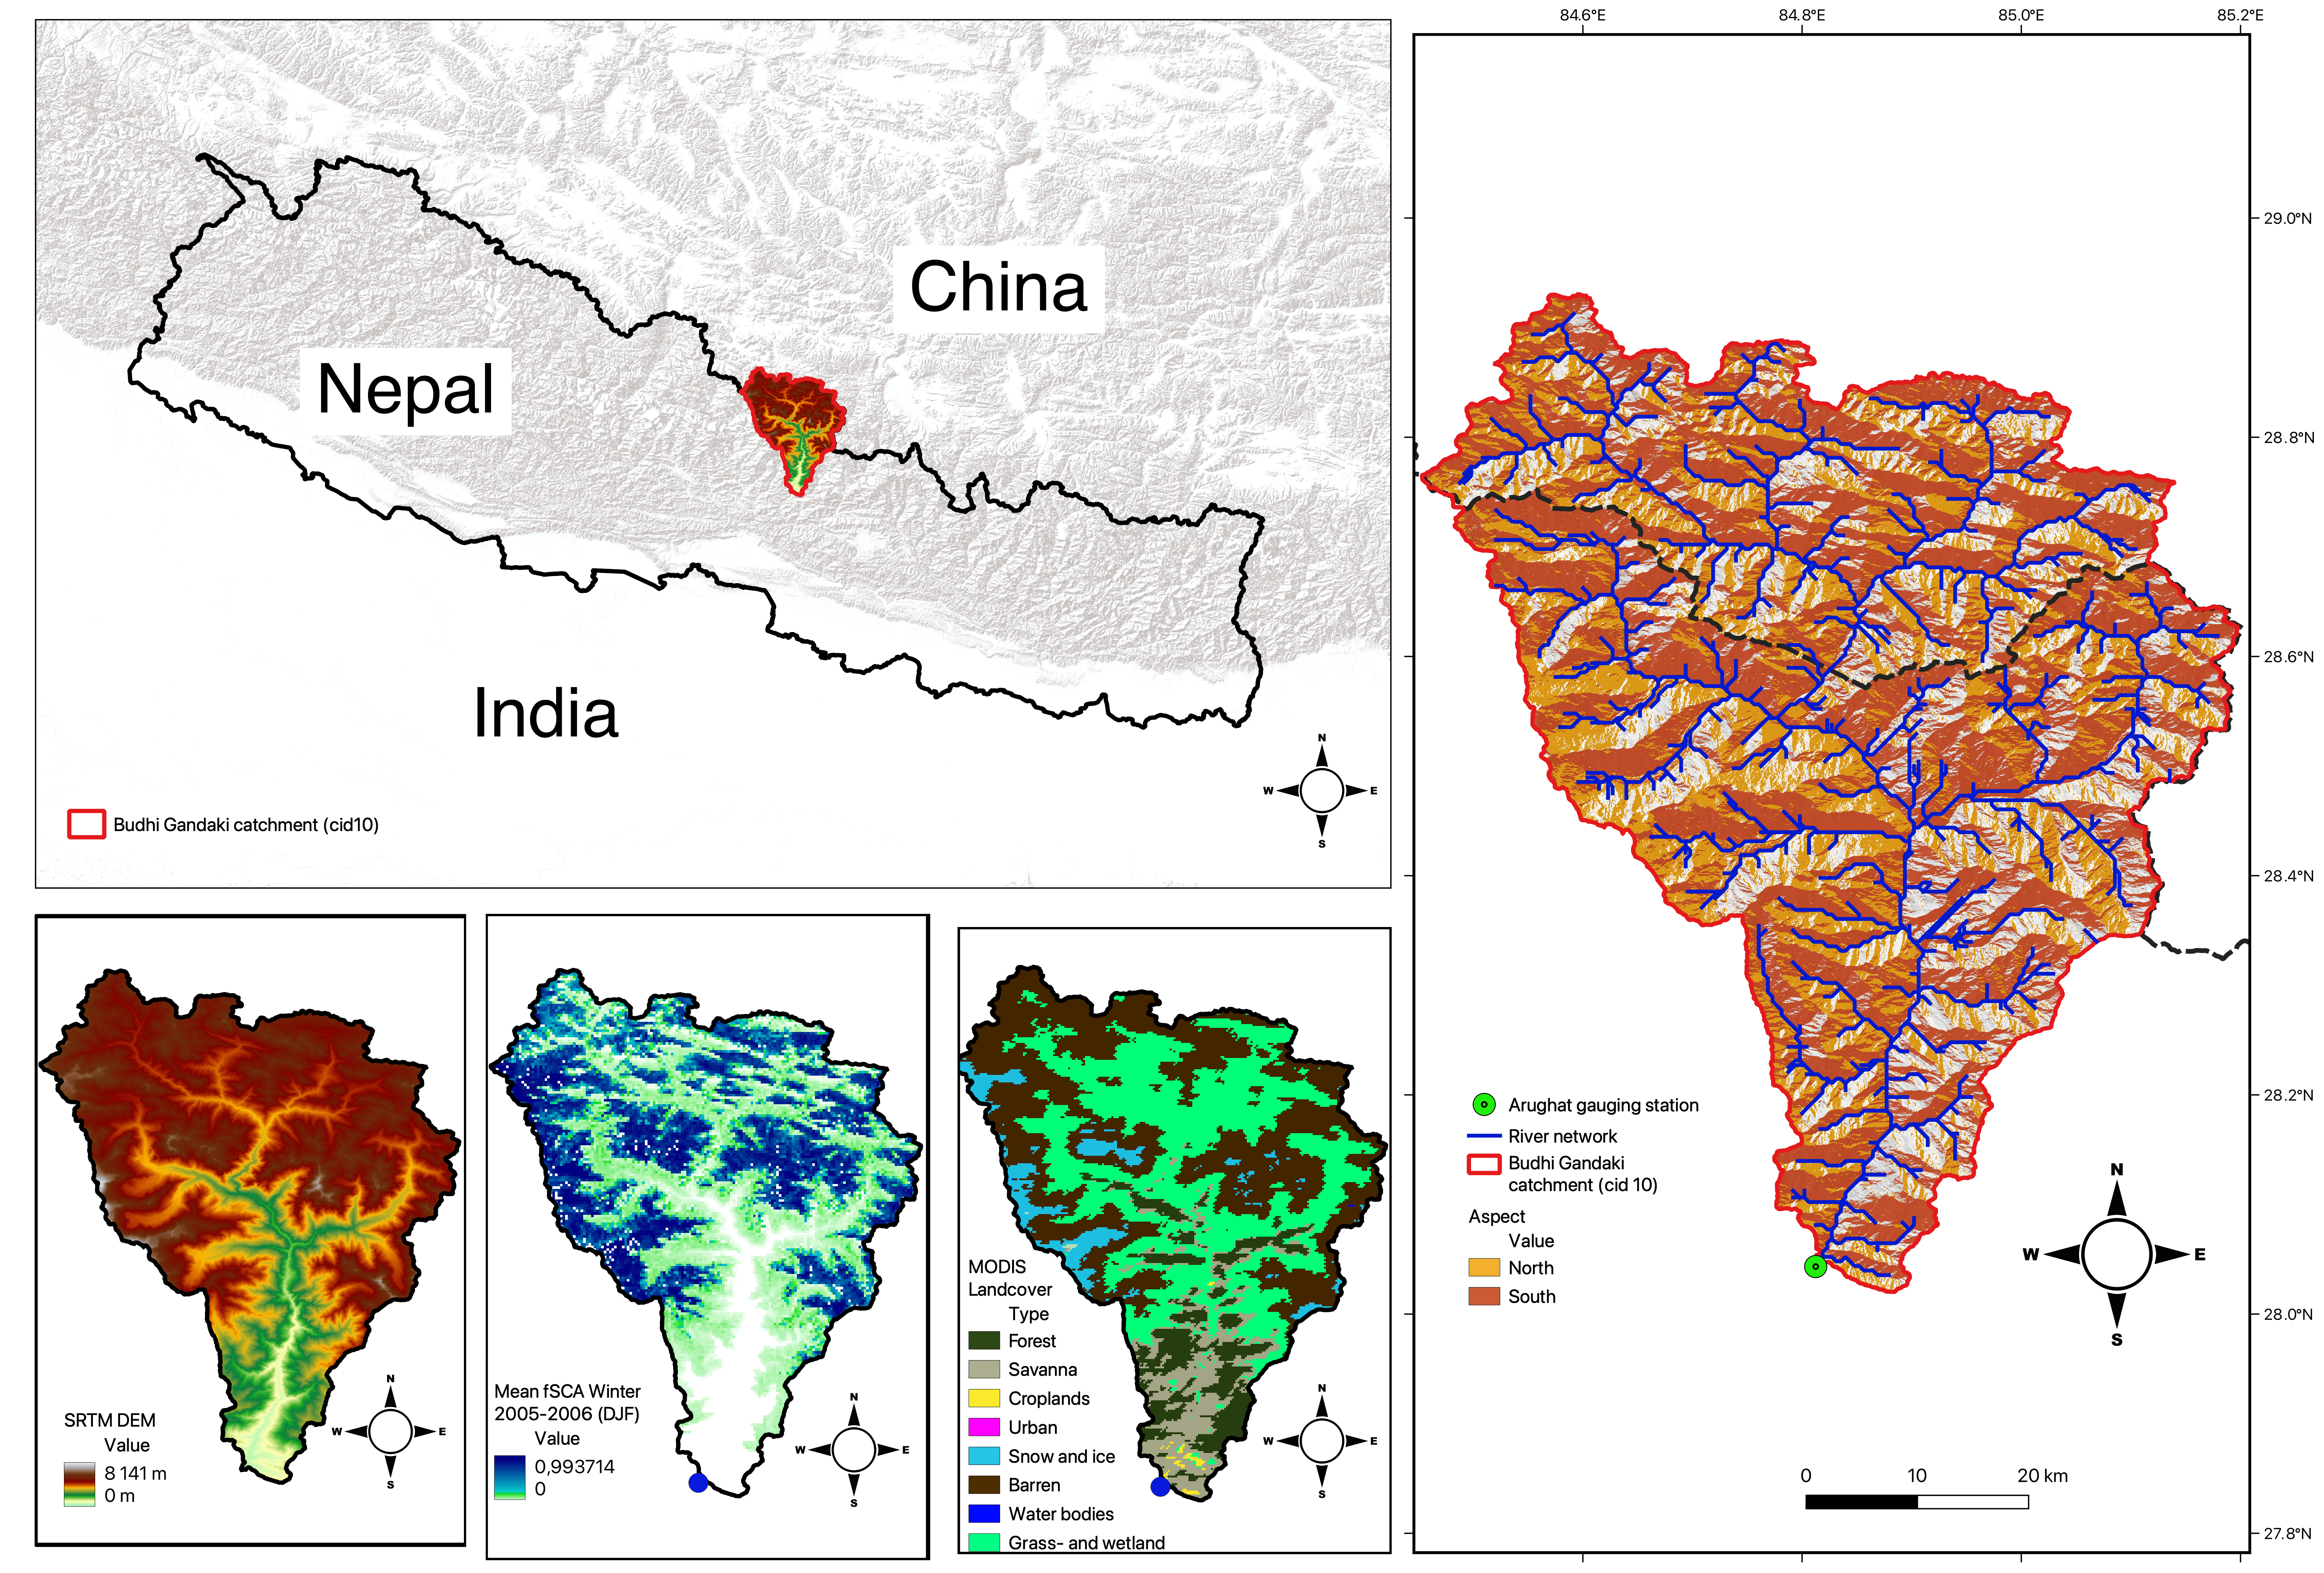
\includegraphics[width=0.8\textwidth]{figures/study_area/overview_map_budhi_gandaki.png}
    \caption{The Budhi Gandaki catchment}
    \label{fig:overview_budhi_gandaki}
\end{figure}


\section{Geography}


The Budhi Gandaki catchment is located in central Nepal (between 27$^{\circ}$50' and 29$^{\circ}$00' N latitudes, and 84$^{\circ}$30' and 85$^{\circ}$10' E longitudes \autocite{marahattaHydrologicalModelingBetter2021}. The catchment is part of the larger Narayani River Catchment originating in Tibet to the north, and is encompassing parts of the Gorkha and Dhading districts of Nepal \autocite{devkotaClimateChangeAdaptation2017}. The Budhi Gandaki catchment is one of the main tributaries of the Trishuli River in Nepal which in turn is a major tributary to the Gandaki River that meets the Ganges in India \autocite{khatriModellingStreamflowSnow2018}. The Budhi Gandaki catchment is about 113 km long and between 15 and 30 km wide \autocite{marahattaHydrologicalModelingBetter2021}. The catchment area upstream of the gauging station at Arughat bazaar is 3871.38 $km^{2}$ \autocite{khatriModellingStreamflowSnow2018}. About 56 $\%$ of the catchment area is in Nepal and 44 $\%$ lies in China. The catchment elevation ranges from green hills (479 m.a.s.l.) at the gauging station in the south to the snow covered Manaslu mountain peak (8029 m.a.s.l.) \autocite{khatriModellingStreamflowSnow2018}. The catchment contains several climatic zones due to the extreme elevation changes within the catchment. The climate changes from tropical (below 1000 m.a.s.l.) to sub-tropical zone (1000 $-$ 2000 m), temperate zone (2000$-$3000 m), subalpine zone (3000$-$4000 m) and alpine zone (4000$-$5000 m) \autocite{khatriModellingStreamflowSnow2018}. The zone above 5000 m is characterized by permanent snow and no human habitation.

\subsection{Hypsograph}

\subsection{Land use}

\section{Climate}

\subsection{Temperature}

The mean temperature ranges from 6 $^{\circ}$C during winter to 35 $^{\circ}$C in summer measured near the Budhi Gandaki Hydropower Project proposed dam site \autocite{devkotaClimateChangeAdaptation2017}. 

\subsection{Prcipitation}
Long-term annual catchment precipitation (1983-2012) is 1301 mm (maximum of 278 mm in July and minimum of 11 mm in November \autocite{marahattaHydrologicalModelingBetter2021}). The annual precipitation varies from greater than 2500 mm at Arughat gauging station to less than 700 mm in the Tibetan part of the catcment \autocite{marahattaHydrologicalModelingBetter2021} The hydrological regime is greatly influenced by the seasons \autocite{bhattaraiEvaluationGlobalForcing2020}. The four seasons are defined as winter (December to February), pre-monsoon (March to May), monsoon (June to September) and post-monsoon (October to November) \autocite{bhattaraiAerosolOpticalDepth2019,shresthaMaximumTemperatureTrends1999}. The catchment receives about 80 $\%$ of the annual precipitation during the monsoon season \autocite{khatriModellingStreamflowSnow2018}. The maximum relative humidity is also reached during the monsoon season. The rainfall decreases from west to east during this period, while the greatest rainfall intensity intensity is occurring on the south facing slopes of the mountains. The catchment is among the tributaries to the Narayani river that are monsoon fed (those in the middle and high mountain regions), in contrast to the glacier and snow melt fed (those originating in a higher Himalayan region) \autocite{bhattaraiEvaluationGlobalForcing2020}.

\subsection{Wind}

\subsection{Relative humidity}

\subsection{Radiation}

\subsection{Snow}

\subsection{Hydrology}
The observed stream flow at Arughat seem to closely follow the precipitation pattern \autocite{marahattaApplicationSWATHydrological2021}. The mean annual flow near the Budhi Gandaki Hydroelectric Project (BGHEP) dam site is estimated at 222 m/s \autocite{dordeFeasibilityStudyDetailed2015}.



\todo[inline]{Percentage of Seasonal PPT, show pie chart}
\todo[inline]{Show annual trends }
\todo[inline]{Monthly average rain days, temperature}
\todo[inline]{Radiation duration}
\todo[inline]{Rating curve}
\todo[inline]{Maximum discharge pr month}
